% Created 2017-04-18 Tue 14:17
% Intended LaTeX compiler: xelatex
\documentclass[a4paper, notitlepage]{report}
\usepackage{graphicx}
\usepackage{grffile}
\usepackage{longtable}
\usepackage{wrapfig}
\usepackage{rotating}
\usepackage[normalem]{ulem}
\usepackage{amsmath}
\usepackage{textcomp}
\usepackage{amssymb}
\usepackage{capt-of}
\usepackage{hyperref}
% set the margins here, if they need to be modified
\usepackage[a4paper, left=1.3in, right=1.0in]{geometry}

% The linespacing you want
\linespread{1.4}

% Lets you pick fonts. Only works if you compile with xelatex or luatex
\usepackage[no-math]{fontspec}

% For block quotes
\usepackage{attrib}

% Additional mathsy symbols
\usepackage{amsmath}
\usepackage{amssymb}

% Used to make the captions on figures sans serif
\usepackage{caption}

% For including images
\usepackage{graphicx}

% For fancy code listings
\usepackage{listings}

% For tables that span multiple pages elegantly
\usepackage{longtable}

% For APA-style citations

% For maintaining a list of abbreviations
\usepackage{nomencl}

% For drawing diagrams
\usepackage{tikz}

% These closely match the SCSS word template fonts
% Won't work unless you compile with xelatex or luatex
\setmainfont[Mapping=tex-text]{Times New Roman}
\setsansfont{Helvetica}
\setmonofont{Courier New}

\pagestyle{headings}

\hypersetup{
    colorlinks,
    citecolor=black,
    filecolor=black,
    linkcolor=black,
    urlcolor=black
}

\bibliographystyle{acm}

% Settings for how you want your code listings to look
\lstset{
basicstyle=\ttfamily\scriptsize,
keywordstyle=\ttfamily,
numberstyle=\rmfamily\tiny,
numbers=left,
commentstyle=\sffamily,
breaklines=true,
frame=single,
stringstyle=\ttfamily,
identifierstyle=\bfseries,
lineskip=1mm
}

% Change these as appropriate, and they'll be filled in automatically on the
% cover page. You can also use them throughout the document, so as not to have
% to type them again all the time.
\newcommand \authorname{Brian McNestry}
\newcommand \authoremail{mcnestrb@tcd.ie}
\newcommand \supervisorname{Dr. Donal O'Mahony}
\newcommand \degreetitle{B.A. (Mod.) Integrated Computer Science}
\newcommand \projecttitle{Electricity Trading Between Smart Nano-Grids: \newline Matching Supply and Demand in the Face of Unpredictable Supply}

% All the commands are defined in this file
\newcommand \inserttitlepage{\thispagestyle{empty}
\begin{center}
{\sffamily
{\Large University of Dublin}

\vspace{10pt}


\includegraphics[scale=0.5]{tcd/trinitycollege.pdf}

\vspace{10pt}

{\Huge TRINITY COLLEGE}

\vspace{80pt}

\textbf{ \Large \emph \projecttitle}

\vspace{30pt}

\authorname

\degreetitle

Final Year Project May 2017

Supervisor: \supervisorname

\vspace{100pt}

\large{School of Computer Science and Statistics
\\$ $\\
O'Reilly Institute, Trinity College, Dublin 2, Ireland}
\linespread{1}
}
\end{center}

}
\newcommand \insertabstract{\begin{abstract}
\thispagestyle{plain}
As fossil fuels across the world are steadily depleted, the majority of the
world's energy production will shift towards renewable sources. However,
renewable energy sources do not always guarantee the same reliability in rates
of production. Therefore new strategies must be developed to match supply and
demand in the face of unpredictable supply. The growing popularity and
proliferation of smart grid technology is one proposed method of solving this
problem.

In this paper, a network implementation of a game theoretic approach to this
problem is implemented in a smart nanogrid to prove whether or not such an
approach is first feasible in a network, and secondly whether or not it would
provide a better approach to the problem. A number of optimisation techniques,
such as convex optimisation and hyperplane projection optimisation, are also
employed to find a better solution. 
\end{abstract}
}
\newcommand \declaration{\chapter*{Declaration}

I hereby declare that this project is entirely my own work and that it has not
been submitted as an exercise for a degree at this or any other university.
$ $\\
$ $\\
\signedanddate
}
\newcommand \acknowledgements{\chapter*{Acknowledgements}

Acknowledge the various people here
}
\newcommand \permissiontolend{\chapter*{Permission to lend}

I agree that the Library and other agents of the College may lend or copy
this report upon request.

$ $\\
$ $\\
\signedanddate
}

\newcommand{\argmax}[1]{\underset{#1}{\operatorname{arg}\,\operatorname{max}}\;}

\usepackage{datetime}

\def\fullhrulefill{\leavevmode\leaders\hrule height 1pt\hfill\kern 0pt}

\newcommand{\signedanddate} {
  \par\noindent\makebox[2.5in]{\fullhrulefill}
  \par\noindent\makebox[2.5in][l]{\authorname, May 5 2017}
}

\newcommand \needcite[1]{\underline{#1}}

\newcommand \abbrev[2]{#1\nomenclature{#1}{#2}}


% For changing the names of the List of Listings, etc.
\renewcommand*{\lstlistlistingname}{List of Listings}
\renewcommand*{\contentsname}{Table of Contents}
\renewcommand*{\nomname}{Abbreviations}

% Make the captions sans serif
\renewcommand{\captionfont}{\sffamily}

\author{Brian McNestry}
\date{\today}
\title{}
\hypersetup{
 pdfauthor={Brian McNestry},
 pdftitle={},
 pdfkeywords={},
 pdfsubject={},
 pdfcreator={Emacs 24.5.1 (Org mode 9.0.5)}, 
 pdflang={English}}
\begin{document}

\inserttitlepage

\pagenumbering{roman}

\declaration

\permissiontolend

\insertabstract

\acknowledgements

\tableofcontents

\newpage


\pagenumbering{arabic}

\part{Abstract}
\label{sec:orgc2b0f77}

\part{Introduction}
\label{sec:org9d885c3}


\part{Background}
\label{sec:org8f3e275}
\chapter{Decentralised Grid}
\label{sec:org468487d}
At present in Ireland and in many other countries, the national electric grid
infrastructure is controlled by a central body, namely the ESB. While there are
several electricity providers in Ireland, such as Bord Gáis Energy, SSE
Airtricity and Energy Ireland, each of them use the same distribution network as
one another. Essentially the power is provided from each of the different
providers and then routed into the same centralised hub belonging to the ESB.
From there, each consumer (a household) receives the energy that they pay for
accordingly at a fixed rate through that same infrastructure belonging to the
ESB. This is much the same system as any other country, where there is a
centralised grid. 

This system has been in place for decades and lends itself very well to the
situation where large companies can provide a steady supply of energy by way of
electricity plants that use both renewable and non-renewable energy sources.
Non-renewable energy sources, also known as fossil fuels, include resources such
as coal, gas and oil. While these are finite resources, at present they can be
burned at a steady rate in order to meet the demands of customers. Electricity
from renewable sources can also be produced at a fairly steady rate by placing
large farms in areas that are particularly well suited to the type of renewable
energy being produced. For example, large wind farms are set up in windy
regions far removed from residential or urban areas and solar panels can be
placed in regions that typically enjoy clearer skies than other areas.

However in the future, perhaps the very near future, with the ongoing depletion
of non-renewable resources, more and more people will turn to deploying solar
panels and local wind farms in their locale, regardless of whether or not they
are living in a particularly sunny or windy area. At the moment there are a few
houses out there that use a solar panel to heat their water or other smaller
tasks but soon more and more people will become more and more dependent on what
they can produce either within their own home, or in a more collective sense in
their own neighbourhood to power their houses.

The issue that then arises in these areas that aren't as sunny or windy is that
supply of electricity is no longer steady. The current system could not be
maintained as the energy produced on a local level would be small enough that it
would not be worth it to pass this energy upstream to the central grid. The
energy would instead be used at a local level to try to cover the demand for
electricity of the house or business with which that particular device is
associated.

The model of infrastructure that would then be required is that of a
decentralised grid. This model would need a massive infrastructure overhaul in
order to implement so it would not exist in the world until it is needed and
accepted by the major companies who would then go about implementing it. In this
case necessity would be the mother of invention, at least on a practical level.
The rough idea of a distributed grid is described in figure 1.1. Throughout the
rest of this report distributed grid and decentralised grid are used
interchangeably. 

\begin{figure}[htbp]
\centering
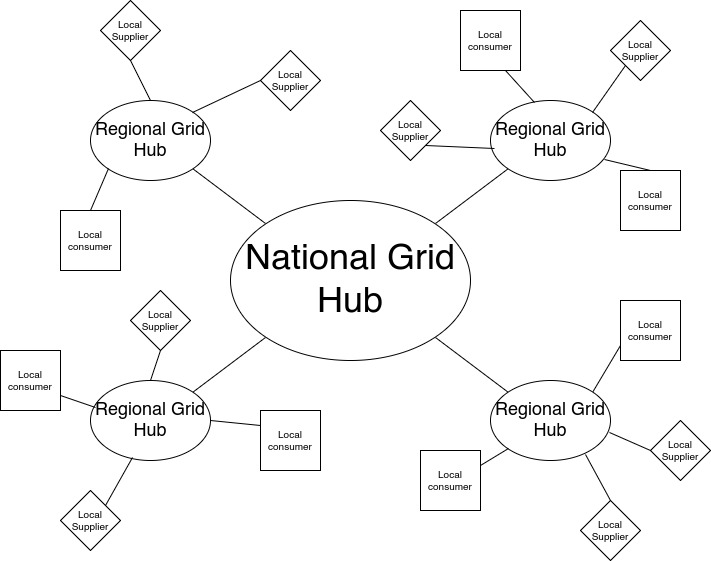
\includegraphics[width=.9\linewidth]{./img/DecentralisedGrid.jpg}
\caption{\label{fig:org9ad2220}
Each local consumer and supplier is attached to a regional grid hub which manages the allocation of electricity between suppliers and consumers. This is just a simple overview of the idea but conceivably a consumer or a supplier could be connected to two or more different regional grid hubs.}
\end{figure}
\chapter{Smart Grid}
\label{sec:org61f0527}
Due to advancements in networking technologies as well as in the field of
sophisticated decision making technologies, the idea of a smart grid has become
increasingly popular. The idea of the smart grid is that actors within a grid,
be they individual consumers or suppliers, or groups thereof, can be fitted with
small computers that perceive changes in the grid and then these actors can
then react accordingly. Several different types of management systems have been
constructed in order to successfully, fairly and efficiently allocate resources
for each of these different types of actors. The two primary types of management
systems that were examined as part of this final year project were Auctions and
Game Theory which will both be discussed in detail later on.

The smart grid is not only used in this regard but in fact has many other
potential applications, some of which have been implemented already in several
cities and regions throughout the world. Other applications of the technology
include energy consumption or production prediction, scheduling the use of
consumers in order to reduce costs or operation and smart reaction and response
to disruptions or blackout within the grid to reduce the damage that occurs as a
result.

In this project it is assumed that the consumers within the system are outfitted
with some kind of prediction technology. An example of such a system has been
proposed by Garcia et al \cite{mohsenian2010optimal} where a device tries to time
its own operation within a certain time-frame in accordance with when the price
of energy is cheapest. It also tries to predict how much energy it will consume
based off its own knowledge of previous experiences in buying power at that
particular time of day, allowing the system to learn over time and make smarter
decisions as time goes on.
\section{Nanogrids}
\label{sec:org42ed8ff}

\chapter{REFIT Scheme}
\label{sec:org58342f2}
\chapter{Auctions}
\label{sec:org139a1e2}


\chapter{Game Theory}
\label{sec:org41c4521}
\section{Cooperative Game Theory}
\label{sec:orgc3b851f}

\section{Non-Cooperative Game Theory}
\label{sec:orgb651563}

\section{Cournot and Stackelberg Games}
\label{sec:org898a4b5}

\chapter{Optimisation Techniques}
\label{sec:org34c25ee}

\section{Convex Optimisation}
\label{sec:orgd480b2f}

\section{Hyperplane Projection}
\label{sec:org7cdb0a2}

\part{Implementation}
\label{sec:orgefa2dd1}

\chapter{Design}
\label{sec:org81c3bed}

\chapter{Framework}
\label{sec:orgc10c3b6}

\chapter{Processes}
\label{sec:org7342f57}

\part{Conclusion}
\label{sec:org63460aa}

\chapter{Assessment}
\label{sec:org0b8dac9}

\chapter{Future Work and Continuations}
\label{sec:orgb29d7df}

\bibliography{bibliography}
\appendix
\end{document}